% Generated by Sphinx.
\def\sphinxdocclass{report}
\documentclass[letterpaper,10pt,openany,oneside]{sphinxmanual}
\usepackage[utf8]{inputenc}
\DeclareUnicodeCharacter{00A0}{\nobreakspace}
\usepackage{cmap}
\usepackage[T1]{fontenc}
\usepackage[english]{babel}
\usepackage{times}
\usepackage[Bjarne]{fncychap}
\usepackage{longtable}
\usepackage{sphinx}
\usepackage{multirow}

        \usepackage{charter}
        \usepackage[defaultsans]{lato}
        \usepackage{inconsolata}
    

\title{NPDL Functional MRI Analysis Manual}
\date{February 22, 2016}
\release{1.0}
\author{Connor Lane}
\newcommand{\sphinxlogo}{
\includegraphics{LabLogo.pdf}\par}
\renewcommand{\releasename}{Release}
\makeindex

\makeatletter
\def\PYG@reset{\let\PYG@it=\relax \let\PYG@bf=\relax%
    \let\PYG@ul=\relax \let\PYG@tc=\relax%
    \let\PYG@bc=\relax \let\PYG@ff=\relax}
\def\PYG@tok#1{\csname PYG@tok@#1\endcsname}
\def\PYG@toks#1+{\ifx\relax#1\empty\else%
    \PYG@tok{#1}\expandafter\PYG@toks\fi}
\def\PYG@do#1{\PYG@bc{\PYG@tc{\PYG@ul{%
    \PYG@it{\PYG@bf{\PYG@ff{#1}}}}}}}
\def\PYG#1#2{\PYG@reset\PYG@toks#1+\relax+\PYG@do{#2}}

\expandafter\def\csname PYG@tok@gd\endcsname{\def\PYG@tc##1{\textcolor[rgb]{0.63,0.00,0.00}{##1}}}
\expandafter\def\csname PYG@tok@gu\endcsname{\let\PYG@bf=\textbf\def\PYG@tc##1{\textcolor[rgb]{0.50,0.00,0.50}{##1}}}
\expandafter\def\csname PYG@tok@gt\endcsname{\def\PYG@tc##1{\textcolor[rgb]{0.00,0.27,0.87}{##1}}}
\expandafter\def\csname PYG@tok@gs\endcsname{\let\PYG@bf=\textbf}
\expandafter\def\csname PYG@tok@gr\endcsname{\def\PYG@tc##1{\textcolor[rgb]{1.00,0.00,0.00}{##1}}}
\expandafter\def\csname PYG@tok@cm\endcsname{\let\PYG@it=\textit\def\PYG@tc##1{\textcolor[rgb]{0.25,0.50,0.56}{##1}}}
\expandafter\def\csname PYG@tok@vg\endcsname{\def\PYG@tc##1{\textcolor[rgb]{0.73,0.38,0.84}{##1}}}
\expandafter\def\csname PYG@tok@m\endcsname{\def\PYG@tc##1{\textcolor[rgb]{0.13,0.50,0.31}{##1}}}
\expandafter\def\csname PYG@tok@mh\endcsname{\def\PYG@tc##1{\textcolor[rgb]{0.13,0.50,0.31}{##1}}}
\expandafter\def\csname PYG@tok@cs\endcsname{\def\PYG@tc##1{\textcolor[rgb]{0.25,0.50,0.56}{##1}}\def\PYG@bc##1{\setlength{\fboxsep}{0pt}\colorbox[rgb]{1.00,0.94,0.94}{\strut ##1}}}
\expandafter\def\csname PYG@tok@ge\endcsname{\let\PYG@it=\textit}
\expandafter\def\csname PYG@tok@vc\endcsname{\def\PYG@tc##1{\textcolor[rgb]{0.73,0.38,0.84}{##1}}}
\expandafter\def\csname PYG@tok@il\endcsname{\def\PYG@tc##1{\textcolor[rgb]{0.13,0.50,0.31}{##1}}}
\expandafter\def\csname PYG@tok@go\endcsname{\def\PYG@tc##1{\textcolor[rgb]{0.20,0.20,0.20}{##1}}}
\expandafter\def\csname PYG@tok@cp\endcsname{\def\PYG@tc##1{\textcolor[rgb]{0.00,0.44,0.13}{##1}}}
\expandafter\def\csname PYG@tok@gi\endcsname{\def\PYG@tc##1{\textcolor[rgb]{0.00,0.63,0.00}{##1}}}
\expandafter\def\csname PYG@tok@gh\endcsname{\let\PYG@bf=\textbf\def\PYG@tc##1{\textcolor[rgb]{0.00,0.00,0.50}{##1}}}
\expandafter\def\csname PYG@tok@ni\endcsname{\let\PYG@bf=\textbf\def\PYG@tc##1{\textcolor[rgb]{0.84,0.33,0.22}{##1}}}
\expandafter\def\csname PYG@tok@nl\endcsname{\let\PYG@bf=\textbf\def\PYG@tc##1{\textcolor[rgb]{0.00,0.13,0.44}{##1}}}
\expandafter\def\csname PYG@tok@nn\endcsname{\let\PYG@bf=\textbf\def\PYG@tc##1{\textcolor[rgb]{0.05,0.52,0.71}{##1}}}
\expandafter\def\csname PYG@tok@no\endcsname{\def\PYG@tc##1{\textcolor[rgb]{0.38,0.68,0.84}{##1}}}
\expandafter\def\csname PYG@tok@na\endcsname{\def\PYG@tc##1{\textcolor[rgb]{0.25,0.44,0.63}{##1}}}
\expandafter\def\csname PYG@tok@nb\endcsname{\def\PYG@tc##1{\textcolor[rgb]{0.00,0.44,0.13}{##1}}}
\expandafter\def\csname PYG@tok@nc\endcsname{\let\PYG@bf=\textbf\def\PYG@tc##1{\textcolor[rgb]{0.05,0.52,0.71}{##1}}}
\expandafter\def\csname PYG@tok@nd\endcsname{\let\PYG@bf=\textbf\def\PYG@tc##1{\textcolor[rgb]{0.33,0.33,0.33}{##1}}}
\expandafter\def\csname PYG@tok@ne\endcsname{\def\PYG@tc##1{\textcolor[rgb]{0.00,0.44,0.13}{##1}}}
\expandafter\def\csname PYG@tok@nf\endcsname{\def\PYG@tc##1{\textcolor[rgb]{0.02,0.16,0.49}{##1}}}
\expandafter\def\csname PYG@tok@si\endcsname{\let\PYG@it=\textit\def\PYG@tc##1{\textcolor[rgb]{0.44,0.63,0.82}{##1}}}
\expandafter\def\csname PYG@tok@s2\endcsname{\def\PYG@tc##1{\textcolor[rgb]{0.25,0.44,0.63}{##1}}}
\expandafter\def\csname PYG@tok@vi\endcsname{\def\PYG@tc##1{\textcolor[rgb]{0.73,0.38,0.84}{##1}}}
\expandafter\def\csname PYG@tok@nt\endcsname{\let\PYG@bf=\textbf\def\PYG@tc##1{\textcolor[rgb]{0.02,0.16,0.45}{##1}}}
\expandafter\def\csname PYG@tok@nv\endcsname{\def\PYG@tc##1{\textcolor[rgb]{0.73,0.38,0.84}{##1}}}
\expandafter\def\csname PYG@tok@s1\endcsname{\def\PYG@tc##1{\textcolor[rgb]{0.25,0.44,0.63}{##1}}}
\expandafter\def\csname PYG@tok@gp\endcsname{\let\PYG@bf=\textbf\def\PYG@tc##1{\textcolor[rgb]{0.78,0.36,0.04}{##1}}}
\expandafter\def\csname PYG@tok@sh\endcsname{\def\PYG@tc##1{\textcolor[rgb]{0.25,0.44,0.63}{##1}}}
\expandafter\def\csname PYG@tok@ow\endcsname{\let\PYG@bf=\textbf\def\PYG@tc##1{\textcolor[rgb]{0.00,0.44,0.13}{##1}}}
\expandafter\def\csname PYG@tok@sx\endcsname{\def\PYG@tc##1{\textcolor[rgb]{0.78,0.36,0.04}{##1}}}
\expandafter\def\csname PYG@tok@bp\endcsname{\def\PYG@tc##1{\textcolor[rgb]{0.00,0.44,0.13}{##1}}}
\expandafter\def\csname PYG@tok@c1\endcsname{\let\PYG@it=\textit\def\PYG@tc##1{\textcolor[rgb]{0.25,0.50,0.56}{##1}}}
\expandafter\def\csname PYG@tok@kc\endcsname{\let\PYG@bf=\textbf\def\PYG@tc##1{\textcolor[rgb]{0.00,0.44,0.13}{##1}}}
\expandafter\def\csname PYG@tok@c\endcsname{\let\PYG@it=\textit\def\PYG@tc##1{\textcolor[rgb]{0.25,0.50,0.56}{##1}}}
\expandafter\def\csname PYG@tok@mf\endcsname{\def\PYG@tc##1{\textcolor[rgb]{0.13,0.50,0.31}{##1}}}
\expandafter\def\csname PYG@tok@err\endcsname{\def\PYG@bc##1{\setlength{\fboxsep}{0pt}\fcolorbox[rgb]{1.00,0.00,0.00}{1,1,1}{\strut ##1}}}
\expandafter\def\csname PYG@tok@kd\endcsname{\let\PYG@bf=\textbf\def\PYG@tc##1{\textcolor[rgb]{0.00,0.44,0.13}{##1}}}
\expandafter\def\csname PYG@tok@ss\endcsname{\def\PYG@tc##1{\textcolor[rgb]{0.32,0.47,0.09}{##1}}}
\expandafter\def\csname PYG@tok@sr\endcsname{\def\PYG@tc##1{\textcolor[rgb]{0.14,0.33,0.53}{##1}}}
\expandafter\def\csname PYG@tok@mo\endcsname{\def\PYG@tc##1{\textcolor[rgb]{0.13,0.50,0.31}{##1}}}
\expandafter\def\csname PYG@tok@mi\endcsname{\def\PYG@tc##1{\textcolor[rgb]{0.13,0.50,0.31}{##1}}}
\expandafter\def\csname PYG@tok@kn\endcsname{\let\PYG@bf=\textbf\def\PYG@tc##1{\textcolor[rgb]{0.00,0.44,0.13}{##1}}}
\expandafter\def\csname PYG@tok@o\endcsname{\def\PYG@tc##1{\textcolor[rgb]{0.40,0.40,0.40}{##1}}}
\expandafter\def\csname PYG@tok@kr\endcsname{\let\PYG@bf=\textbf\def\PYG@tc##1{\textcolor[rgb]{0.00,0.44,0.13}{##1}}}
\expandafter\def\csname PYG@tok@s\endcsname{\def\PYG@tc##1{\textcolor[rgb]{0.25,0.44,0.63}{##1}}}
\expandafter\def\csname PYG@tok@kp\endcsname{\def\PYG@tc##1{\textcolor[rgb]{0.00,0.44,0.13}{##1}}}
\expandafter\def\csname PYG@tok@w\endcsname{\def\PYG@tc##1{\textcolor[rgb]{0.73,0.73,0.73}{##1}}}
\expandafter\def\csname PYG@tok@kt\endcsname{\def\PYG@tc##1{\textcolor[rgb]{0.56,0.13,0.00}{##1}}}
\expandafter\def\csname PYG@tok@sc\endcsname{\def\PYG@tc##1{\textcolor[rgb]{0.25,0.44,0.63}{##1}}}
\expandafter\def\csname PYG@tok@sb\endcsname{\def\PYG@tc##1{\textcolor[rgb]{0.25,0.44,0.63}{##1}}}
\expandafter\def\csname PYG@tok@k\endcsname{\let\PYG@bf=\textbf\def\PYG@tc##1{\textcolor[rgb]{0.00,0.44,0.13}{##1}}}
\expandafter\def\csname PYG@tok@se\endcsname{\let\PYG@bf=\textbf\def\PYG@tc##1{\textcolor[rgb]{0.25,0.44,0.63}{##1}}}
\expandafter\def\csname PYG@tok@sd\endcsname{\let\PYG@it=\textit\def\PYG@tc##1{\textcolor[rgb]{0.25,0.44,0.63}{##1}}}

\def\PYGZbs{\char`\\}
\def\PYGZus{\char`\_}
\def\PYGZob{\char`\{}
\def\PYGZcb{\char`\}}
\def\PYGZca{\char`\^}
\def\PYGZam{\char`\&}
\def\PYGZlt{\char`\<}
\def\PYGZgt{\char`\>}
\def\PYGZsh{\char`\#}
\def\PYGZpc{\char`\%}
\def\PYGZdl{\char`\$}
\def\PYGZhy{\char`\-}
\def\PYGZsq{\char`\'}
\def\PYGZdq{\char`\"}
\def\PYGZti{\char`\~}
% for compatibility with earlier versions
\def\PYGZat{@}
\def\PYGZlb{[}
\def\PYGZrb{]}
\makeatother

\renewcommand\PYGZsq{\textquotesingle}

\begin{document}

\maketitle
\tableofcontents
\phantomsection\label{index::doc}



\chapter{Data organization}
\label{data_organization:data-organization}\label{data_organization::doc}\label{data_organization:welcome-to-npdl-functional-mri-analysis-manual-s-documentation}

\section{Exploring the Godzilla server}
\label{data_organization:exploring-the-godzilla-server}
Once data is collected, it's sent to the KKI Godzilla server for permanent
storage. The first step in analysis then is to retrieve the data from Godzilla.
Like our lab server, Godzilla is a UNIX machine, so we will use standard
command line tools to log onto the server and transfer data.

To log onto the server, you need to contact system administrator at KKI and
request an account. When you have an account, you can log on using \code{ssh} and
begin exploring.

To simplify the log-in process, you should set up public key authentication.
For a description of what this is and how to do it, see \href{https://macnugget.org/projects/publickeys/}{this tutorial}\footnote{https://macnugget.org/projects/publickeys/}.

Once you're logged in, navigate to /g4/mbedny. This is our lab folder on
Godzilla. All of our studies are stored in this folder (e.g. BSYN, BRAILLE).
Within each study folder, there will be a folder for each subject. And within
each subject's folder, a par and rec file for each collected run, plus
an MR folder, containing DICOM images for the MPRAGE scan:

\begin{Verbatim}[commandchars=\\\{\}]
/g4/mbedby/
  \textbar{}\PYGZhy{} BSYN/
    \textbar{}\PYGZhy{} BSYN\PYGZus{}S\PYGZus{}01/
      \textbar{}\PYGZhy{} bsyn\PYGZus{}s\PYGZus{}01\PYGZus{}3\PYGZus{}1.par
      \textbar{}\PYGZhy{} bsyn\PYGZus{}s\PYGZus{}01\PYGZus{}3\PYGZus{}1.rec
      \textbar{}\PYGZhy{} bsyn\PYGZus{}s\PYGZus{}01\PYGZus{}4\PYGZus{}1.par
      \textbar{}\PYGZhy{} bsyn\PYGZus{}s\PYGZus{}01\PYGZus{}4\PYGZus{}1.rec
    \textbar{}\PYGZhy{} BSYN\PYGZus{}S\PYGZus{}02/
  \textbar{}\PYGZhy{} BRAILLE1/
    \textbar{}\PYGZhy{} BRAILLE1\PYGZus{}CB\PYGZus{}01
      \textbar{}\PYGZhy{} MR/
        \textbar{}\PYGZhy{} 1.3.46.670589.11.24058.5.0.1788.2014053014171806001
        \textbar{}\PYGZhy{} 1.3.46.670589.11.24058.5.0.1788.2014053014171865002
      \textbar{}\PYGZhy{} braille1\PYGZus{}cb\PYGZus{}01\PYGZus{}3\PYGZus{}1.par
      \textbar{}\PYGZhy{} braille1\PYGZus{}cb\PYGZus{}01\PYGZus{}3\PYGZus{}1.rec
\end{Verbatim}

Typically, runs 1, 2 are the survey and reference scans respectively. These
scans are not usually sent to Godzilla during data collection. The first scan
we keep is usually run 3, the MPRAGE.


\section{The scan log}
\label{data_organization:the-scan-log}
For each scanning session you must keep a scan log documenting the events of
the session. The scan log is how we associate scanner runs with behavioral
files. Without the scan logs we could not run any analyses.

You should keep both a written scan log and an electronic version. The format
for the electronic version is as follows:

\begin{Verbatim}[commandchars=\\\{\}]
\PYGZsh{} Study: BSYN
\PYGZsh{} Subject ID: BSYN\PYGZus{}S\PYGZus{}01
\PYGZsh{} Scanner ID: BSYN\PYGZus{}04
\PYGZsh{} Registration ID: 1403250900
\PYGZsh{} Date: 3/25/14 9:00
\PYGZsh{} Scanner: MR1 32ch
\PYGZsh{} Scanned by: TB

3 mprage
4 bsyn\PYGZus{}01
5 bsyn\PYGZus{}02
6 bsyn\PYGZus{}03
7 bsyn\PYGZus{}04 \PYGZsh{} participant got out to use the restroom.
8 bsyn\PYGZus{}05
9 bsyn\PYGZus{}06

\PYGZsh{} Notes:
\PYGZsh{} \PYGZhy{} Volume set to 2.5
\PYGZsh{} \PYGZhy{} Good performance on average
\PYGZsh{} \PYGZhy{} Subject a little claustrophobic for the first scan
\end{Verbatim}

The scan log starts with a header containing info about the scan session: the
study name, the subject ID, the scanner subject ID (which may or may not be
different), etc.
\begin{itemize}
\item {} 
Each line of the header must start with ``\#''.

\item {} 
The ``key'' for each line must be spelled exactly as shown.

\item {} 
The keys must be separated from their values with a colon.

\end{itemize}

The next section of the scan log is a two-column matrix consisting of run
number, run name pairs. The run number is the number of the scan, as it was
collected. The run name typically has the format \code{\{task\}\_\{run num\}}, with the
run number being zero-padded to two places.

Last, there is an optional \emph{Notes} section, where you can record miscellaneous
information about the session or the participant. Each line of notes should
start with ``\#''.


\section{Transferring data for analysis}
\label{data_organization:transferring-data-for-analysis}
Transferring data is a three part process:
\begin{enumerate}
\item {} 
Fetch the par and rec files from Godzilla.

\item {} 
Convert the par/recs to gzipped Nifti files.

\item {} 
Rename the converted files to something more convenient than the default
scanner names.

\end{enumerate}

All of these steps are accomplished with the \code{parfetch} command, which is
part of the lab's suite of scripts

\begin{Verbatim}[commandchars=\\\{\}]
Usage: parfetch [options] \PYGZlt{}scan\PYGZhy{}log\PYGZgt{}

Fetch par and rec files from the scanner file server and convert
to gzipped nifti. File organization on the server is assumed to
follow the convention:

  \PYGZob{}lab dir\PYGZcb{}/\PYGZob{}study dir\PYGZcb{}/\PYGZob{}subject ID\PYGZcb{}/*\PYGZus{}\PYGZob{}run \PYGZsh{}\PYGZcb{}\PYGZus{}\PYGZob{}acq \PYGZsh{}\PYGZcb{}.*

Arguments:
  \PYGZlt{}scan\PYGZhy{}log\PYGZgt{}   Scan log text file. Describes how files should be
               renamed. First column is run number, second column
               is new name. You may optionally specify the Study,
               Subject ID, and/or Scanner ID in a comment line
               (starting with \PYGZsh{}). All other lines starting with \PYGZsh{}
               will be ignored. See below for an example of the
               proper format.

Options:
  \PYGZhy{}\PYGZhy{}study \PYGZlt{}study\PYGZgt{}     Name of study on server. Read from the scan log
                      by default (needs a \PYGZsq{}\PYGZsh{} Study: XXXX\PYGZsq{} line).
  \PYGZhy{}\PYGZhy{}sub \PYGZlt{}scan\PYGZhy{}sub\PYGZgt{}    Scanner subject ID on server. Read from the scan
                      log by default (needs a \PYGZsq{}\PYGZsh{} Scanner ID: XXXX\PYGZsq{} line).
  \PYGZhy{}\PYGZhy{}out \PYGZlt{}outdir\PYGZgt{}      Directory to put converted data. If this option
                      is not specified, the converted data will be placed
                      in \PYGZob{}subject ID\PYGZcb{}/raw, in the working directory,
                      where \PYGZob{}subject ID\PYGZcb{} is read from the scan log.
  \PYGZhy{}\PYGZhy{}u \PYGZlt{}user\PYGZgt{}          Name of server user [default: clane9].
  \PYGZhy{}\PYGZhy{}labdir \PYGZlt{}dir\PYGZgt{}      Lab directory on server [default: /g4/mbedny].
  \PYGZhy{}\PYGZhy{}no\PYGZhy{}clean          Don\PYGZsq{}t delete redundant rec files.
\end{Verbatim}

First \code{parfetch} reads the scan log for the scan session to determine where
the data is located on Godzilla, and where it should be placed on the lab
server. It uses the ``Study'' and ``Scanner ID'' values to determine where the data
is located, and it uses the ``Subject ID'' value to decide where to put the data
(defaulting to \code{\{Subject ID\}/raw} in the working directory.

Next, the command transfers the data to the lab server using the \code{scp}
command. For this part to work it is essential that you can access Godzilla.
And if you have public-key authentication set up, you won't have to enter your
password. Next, \code{parfetch} uses \code{dcm2nii} to convert the data to gzipped
Nifti files. See the \href{http://www.mccauslandcenter.sc.edu/mricro/mricron/dcm2nii.html}{Mricron}\footnote{http://www.mccauslandcenter.sc.edu/mricro/mricron/dcm2nii.html} site for details on this part. Last, \code{parfetch}
renames the converted files according to the names given in the second column
in the scan log.

If we were to run \code{parfetch} on the example scan log above, the resulting raw
folder would be structured like this:

\begin{Verbatim}[commandchars=\\\{\}]
BSYN\PYGZus{}S\PYGZus{}01/
  \textbar{}\PYGZhy{} raw/
    \textbar{}\PYGZhy{} bsyn\PYGZus{}01.nii.gz
    \textbar{}\PYGZhy{} bsyn\PYGZus{}02.nii.gz
    \textbar{}\PYGZhy{} mprage.nii.gz
    \textbar{}\PYGZhy{} par/
      \textbar{}\PYGZhy{} bsyn\PYGZus{}04\PYGZus{}3\PYGZus{}1.par
      \textbar{}\PYGZhy{} bsyn\PYGZus{}04\PYGZus{}4\PYGZus{}1.par
      \textbar{}\PYGZhy{} MR/
    \textbar{}\PYGZhy{} parfetch.log
    \textbar{}\PYGZhy{} sl.txt
\end{Verbatim}


\chapter{Surface reconstruction}
\label{surface_reconstruction:surface-reconstruction}\label{surface_reconstruction::doc}\label{surface_reconstruction:mricron}

\section{Surfaces}
\label{surface_reconstruction:surfaces}
Most of our analyses are performed on data that have been mapped to the
cortical surface. Surface-based data files come in mainly two kinds: anatomical
surfaces, and metric overlays. Anatomical surfaces are like high-res T1 images.
They are used to represent the shape of the cortical sheet, all of the sulci
and gyri. Anatomical surfaces are geometrical structures made up of triangular
faces that are ``glued'' together along the edges to form a closed ``mesh''. The
points of the triangular faces are called vertices. Vertices are the surface
analogues to voxels. They are the units of analysis.
\begin{figure}[htbp]
\centering
\capstart

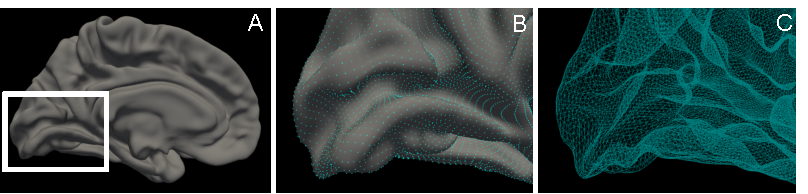
\includegraphics{surf_mesh_01.pdf}
\caption{Renderings of an anatomical surface. \textbf{(A)} The entire surface shown from
the medial view. V1 is boxed. \textbf{(B)} A close-up of V1, with vertices shown
in teal. \textbf{(C)} Another close-up of V1, this time showing the mesh structure.}\end{figure}

Metric overlays, on the other hand, are more like BOLD images. Metrics store
the actual functional data. At bottom, metrics are mappings between the
vertices of an anatomical surface and some numerical data. The numerical data
assigned to each vertex can either be a vector, like a functional time series,
or a single scalar, such as a \emph{z} or \emph{t} value. Metrics are also commonly used
to represent ROIs, by assigning vertices within the ROI the value 1, and all
other vertices 0. One important thing to remember is that metrics contain no
anatomical structure. This is unlike standard BOLD images, where the spatial
relationships between data points are encoded in the file format itself.
\begin{figure}[htbp]
\centering
\capstart

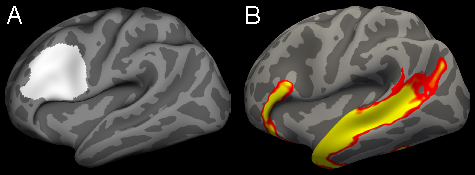
\includegraphics{metrics_01.pdf}
\caption{Examples of metric overlays. \textbf{(A)} An ROI in inferior frontal cortex,
represented with 1's and 0's. \textbf{(B)} A \emph{z}-stat image for a language contrast.}\end{figure}


\section{Introduction to Freesurfer}
\label{surface_reconstruction:introduction-to-freesurfer}
All of our surface-based analyses depend a lot on the Freesurfer software
package. Freesurfer is basically a set of command-line tools for generating and
manipulating surface files. Generating anatomical surfaces from T1 images is
probably the most important thing we use Freesurfer for. The command for that
is called \code{recon-all}. Some other important uses for Freesurfer include:
\begin{itemize}
\item {} 
Volume and surface visualization (\href{http://freesurfer.net/fswiki/FreeviewGuide}{freeview}\footnote{http://freesurfer.net/fswiki/FreeviewGuide}, \href{https://surfer.nmr.mgh.harvard.edu/fswiki/tksurfer}{tksurfer}\footnote{https://surfer.nmr.mgh.harvard.edu/fswiki/tksurfer})

\item {} 
Volume and surface file conversion (\code{mri\_convert}, \code{mris\_convert})

\item {} 
Surface-informed volume registration (\code{bbregister})

\item {} 
Surface manipulation (\code{mri\_surf2surf})

\item {} 
Surface-based group fMRI statsistics (\code{mri\_glmfit})

\end{itemize}

Freesurfer uses a centralized workspace called the \emph{Subjects Directory} for
carrying out most of its processing. The location of the Subjects Directory is
determined by the shell environment variable \code{SUBJECTS\_DIR}. Within the
Subjects Directory there are going to be many individual \emph{subject folders}.
These folders are generated when you run \code{recon-all}. Their purpose is to
store all of the output surface files and intermediate volume files created by
\code{recon-all}. For example, the default Freesurfer Subjects Directory
(\code{\$FREESURFER\_HOME/subjects}), contains a subject called ``bert'':

\begin{Verbatim}[commandchars=\\\{\}]
bert/
  \textbar{}\PYGZhy{} bem/
  \textbar{}\PYGZhy{} label/
  \textbar{}\PYGZhy{} mri/
    \textbar{}\PYGZhy{} brain.mgz
    \textbar{}\PYGZhy{} orig.mgz
    \textbar{}\PYGZhy{} T1.mgz
  \textbar{}\PYGZhy{} scripts/
    \textbar{}\PYGZhy{} recon\PYGZhy{}all.log
    \textbar{}\PYGZhy{} recon\PYGZhy{}all\PYGZhy{}status.log
  \textbar{}\PYGZhy{} src/
  \textbar{}\PYGZhy{} stats/
  \textbar{}\PYGZhy{} surf/
    \textbar{}\PYGZhy{} lh.pial
    \textbar{}\PYGZhy{} rh.pial
    \textbar{}\PYGZhy{} lh.sphere.reg
    \textbar{}\PYGZhy{} rh.sphere.reg
    \textbar{}\PYGZhy{} lh.white
    \textbar{}\PYGZhy{} rh.white
  \textbar{}\PYGZhy{} tmp/
  \textbar{}\PYGZhy{} touch/
  \textbar{}\PYGZhy{} trash/
\end{Verbatim}

The mri and surf folders contain the output volume and surface files
respectively. For example, T1.mgz is a copy of the raw T1 volume, after
intensity bias correction has been applied. lh.white is an anatomical
surface that follows the grey/white matter boundary in the left hemisphere.

\begin{notice}{note}{Note:}
Freesurfer uses a custom file format to represent MRI volumes and
surfaces. These files usually have the extension \code{.mgh} or \code{.mgz}
(compressed). You can convert these files to more standard formats
like Nifti and Gifti using \code{mri\_convert} and \code{mris\_convert}
respectively.
\end{notice}

A good way to get familiar with all of the Freesurfer output files is by
following the \href{http://freesurfer.net/fswiki/FsTutorial/OutputData\_freeview}{Freesurfer output inspection tutorial}\footnote{http://freesurfer.net/fswiki/FsTutorial/OutputData\_freeview}, either with the
tutorial data or your own. This is also a good way to get familiar with the
primary Freesurfer visualization tool, \href{http://freesurfer.net/fswiki/FreeviewGuide}{freeview}\footnote{http://freesurfer.net/fswiki/FreeviewGuide}.

When you open a new terminal, \code{SUBJECTS\_DIR} will probably be set to
\code{\$NPDL\_SCRIPT\_DIR/subjects}. This is a lab-specific folder that contains the
three \emph{group average} subjects we use most often: fsaverage, 32k\_fs\_LR, and
164k\_fs\_LR. fsaverage comes packaged with Freesurfer and is based on the MNI
305 template. 164k\_fs\_LR and 32k\_fs\_LR are derived from it. It is useful to
have the \code{SUBJECTS\_DIR} set this way, so you can have easy access to these
subject folders. However, when it is time for you to do your own analyses, you
will need to create a Subjects Directory inside your analysis folder to hold
the surface reconstruction folders for your study subjects.


\subsection{Additional Freesurfer resources}
\label{surface_reconstruction:additional-freesurfer-resources}\begin{itemize}
\item {} 
The Freesurfer course materials: \href{https://surfer.nmr.mgh.harvard.edu/fswiki/FsTutorial}{https://surfer.nmr.mgh.harvard.edu/fswiki/FsTutorial}

\item {} 
The Freesurfer youtube channel: \href{https://www.youtube.com/channel/UCruQerP8aa-gYttXkAcyveA}{https://www.youtube.com/channel/UCruQerP8aa-gYttXkAcyveA}
\begin{itemize}
\item {} 
In particular, the smoothing and registration talk, which is all about the
benefits of surface-based analysis: \href{https://www.youtube.com/watch?v=8WPvXoORoAw}{https://www.youtube.com/watch?v=8WPvXoORoAw}

\end{itemize}

\end{itemize}


\section{Running \texttt{recon-all}}
\label{surface_reconstruction:running-recon-all}\label{surface_reconstruction:freesurfer-output-inspection-tutorial}
Freesurfer's entire surface reconstruction pipeline is completely automated. It
only takes one command to get the process going, e.g.:

\begin{Verbatim}[commandchars=\\\{\}]
recon\PYGZhy{}all \PYGZhy{}subject BLAH\PYGZus{}S\PYGZus{}01 \PYGZhy{}i T1.nii.gz \PYGZhy{}all
\end{Verbatim}

This command will create a subject folder called BLAH\_S\_01 inside the Subjects
Directory and begin populating it with BLAH\_S\_01's anatomical surfaces. The
only input is T1.nii.gz, the high resolution T1 volume. There are about 34
steps in the entire processing stream, starting with intensity normalization
and skull stripping, and going through surface creation, surface inflation, and
surface-based registration to fsaverage. Altogether it can take up to 10 hours
to complete (on our machine it's usually about 6 hours). The \code{-all} option
tells recon-all to do all 34 steps.

You can view the complete description of all processing steps either by looking
at the \code{recon-all} help message, or by navigating to the online \href{http://freesurfer.net/fswiki/FreeSurferAnalysisPipelineOverview}{Freesurfer
analysis pipeline overview}\footnote{http://freesurfer.net/fswiki/FreeSurferAnalysisPipelineOverview}. If you're looking for more detail, try the
\href{http://freesurfer.net/fswiki/ReconAllTableStableV5.3}{recon-all table}\footnote{http://freesurfer.net/fswiki/ReconAllTableStableV5.3} which contains a complete outline of all the reconstruction
steps, and the sub-commands involved.

\begin{notice}{note}{Note:}
Make sure to set the \code{SUBJECTS\_DIR} environment variable properly
before you start your analyses. Otherwise \code{recon-all} will try to write to
the default Subjects Directory, which will likely cause a permissions error.
\end{notice}


\section{Inspecting outputs}
\label{surface_reconstruction:recon-all-table}\label{surface_reconstruction:inspecting-outputs}
The critical outputs of the Freesurfer reconstruction process are four surfaces
(two for each hemisphere). The left and right ``white'' surfaces mark the
grey/white matter boundary. The left and right ``pial'' surfaces mark the
CSF/grey matter boundary. The goal of data inspection is to check that the
volume between these surfaces includes all and only grey matter.

We visually inspect these surfaces overlaid onto the high-res anatomical image.
To do this, we load the surfaces and the high-res anatomical into the
Freesurfer viewer, \href{http://freesurfer.net/fswiki/FreeviewGuide}{freeview}\footnote{http://freesurfer.net/fswiki/FreeviewGuide}. Freeview can be opened at the terminal by typing
\code{freeview}. You can then use the GUI interface to load the surfaces and T1
image.

Alternatively, you can specify the images as command-line arguments to the
\code{freeview} command.

To make loading images easier, we have the command \code{checksurf}, which only
requires a subject ID argument (provided the \code{SUBJECTS\_DIR} is set properly):

\begin{Verbatim}[commandchars=\\\{\}]
checksurf \PYG{n+nv}{\PYGZdl{}subj}
\end{Verbatim}

All \code{checksurf} does is encapsulate what would be a very long \code{freeview}
call: loading the original T1, the brain-extracted T1, the left and right white
and pial surfaces, as well as the left and right inflated surfaces

\begin{Verbatim}[commandchars=\\\{\}]
freeview \PYG{l+s+se}{\PYGZbs{}}
  \PYGZhy{}v \PYG{l+s+se}{\PYGZbs{}}
  \PYG{n+nv}{\PYGZdl{}SUBJECTS\PYGZus{}DIR}/\PYG{n+nv}{\PYGZdl{}subj}/mri/brainmask.mgz \PYG{l+s+se}{\PYGZbs{}}
  \PYG{n+nv}{\PYGZdl{}SUBJECTS\PYGZus{}DIR}/\PYG{n+nv}{\PYGZdl{}subj}/mri/orig.mgz:visible\PYG{o}{=}0 \PYG{l+s+se}{\PYGZbs{}}
  \PYGZhy{}f \PYG{l+s+se}{\PYGZbs{}}
  \PYG{n+nv}{\PYGZdl{}SUBJECTS\PYGZus{}DIR}/\PYG{n+nv}{\PYGZdl{}subj}/surf/lh.white:edgecolor\PYG{o}{=}blue:edgethickness\PYG{o}{=}2 \PYG{l+s+se}{\PYGZbs{}}
  \PYG{n+nv}{\PYGZdl{}SUBJECTS\PYGZus{}DIR}/\PYG{n+nv}{\PYGZdl{}subj}/surf/rh.white:edgecolor\PYG{o}{=}blue:edgethickness\PYG{o}{=}2 \PYG{l+s+se}{\PYGZbs{}}
  \PYG{n+nv}{\PYGZdl{}SUBJECTS\PYGZus{}DIR}/\PYG{n+nv}{\PYGZdl{}subj}/surf/lh.pial:edgecolor\PYG{o}{=}green:edgethickness\PYG{o}{=}2 \PYG{l+s+se}{\PYGZbs{}}
  \PYG{n+nv}{\PYGZdl{}SUBJECTS\PYGZus{}DIR}/\PYG{n+nv}{\PYGZdl{}subj}/surf/rh.pial:edgecolor\PYG{o}{=}green:edgethickness\PYG{o}{=}2 \PYG{l+s+se}{\PYGZbs{}}
  \PYG{n+nv}{\PYGZdl{}SUBJECTS\PYGZus{}DIR}/\PYG{n+nv}{\PYGZdl{}subj}/surf/lh.inflated:edgethickness\PYG{o}{=}0:visible\PYG{o}{=}0 \PYG{l+s+se}{\PYGZbs{}}
  \PYG{n+nv}{\PYGZdl{}SUBJECTS\PYGZus{}DIR}/\PYG{n+nv}{\PYGZdl{}subj}/surf/rh.inflated:edgethickness\PYG{o}{=}0:visible\PYG{o}{=}0
\end{Verbatim}

To check the surface boundaries, you will want to scroll through each slice of
the image, looking for places where too much or too little has been included as
``grey matter''. You should pick either the sagittal, coronal, or axial view from
the top menu bar, and work your way through the entire image. You can scroll
the slices using ``Fn+Up Arrow'' and ``Fn+Down Arrow''. Some other useful shortcuts
are:
\begin{itemize}
\item {} 
Shift+Left click drag: Control brightness/contrast of the anatomical image

\item {} 
Mouse scroll: Zoom in/out

\item {} 
Ctrl+Left click: Zoom in at cursor

\item {} 
Ctrl+Right click: Zoom out at cursor

\item {} 
Left/Right/Up/Down Arrow: Move FOV

\end{itemize}

These shortcuts and others can also be found in Help --\textgreater{} Quick Reference in
the Freeview window.

Some general pointers for checking surface accuracy:
\begin{itemize}
\item {} 
About 1-3 seconds per slice tends to be a good pace.

\item {} 
I prefer to holistically watch the entire cortex as I scroll through, rather
than fixate on each individual sulcus and gyrus.

\item {} 
When you see something that doesn't look right, try clicking on the spot and
changing views. Getting a different perspective usually helps you decide if
what you're seeing is really an error.

\item {} 
It also helps to pass over a problem area a few times, scrolling back and
forth. Getting a better idea of the context around a potential reconstruction
error will usually help you decide what to do about it.

\end{itemize}


\section{Common reconstruction errors}
\label{surface_reconstruction:common-reconstruction-errors}\label{surface_reconstruction:id1}
Most of the time the surfaces produced by Freesurfer are just fine and don't
need any intervention (say \textasciitilde{}50\% of subjects). When there are surface
problems, they'll usually fall into one of the following categories.

\begin{notice}{note}{Note:}
Many of these errors are covered in the \href{http://surfer.nmr.mgh.harvard.edu/pub/docs/freesurfer\_failuremodes\_ani.ppt}{Freesurfer failure modes
talk}\footnote{http://surfer.nmr.mgh.harvard.edu/pub/docs/freesurfer\_failuremodes\_ani.ppt},
and the fixes are described in the \href{https://surfer.nmr.mgh.harvard.edu/fswiki/FsTutorial/TroubleshootingData}{Freesurfer troubleshooting tutorial}\footnote{https://surfer.nmr.mgh.harvard.edu/fswiki/FsTutorial/TroubleshootingData}.
\textbf{When unsure, defer!} Freesurfer is smart, and objective. If you're
not sure that what you're seeing is an error, just let it be.
\end{notice}


\subsection{Bad white matter segmentation}
\label{surface_reconstruction:bad-white-matter-segmentation}
The segmentation of white matter from grey matter relies on white matter voxels
having a consistent intensity. When you get a region of white matter that is
especially bright or dark, this can cause Freesurfer to mislabel it. You'll
often see this problem in the long, thin gyri located in anterior temporal
lobe.

To fix this kind of error, you'll need to place some \emph{control points} on or
around the mislabeled voxels, and re-run \code{recon-all}. For a full description
of the steps to take, see the \href{https://surfer.nmr.mgh.harvard.edu/fswiki/FsTutorial/ControlPoints\_freeview}{Freesurfer control points tutorial}\footnote{https://surfer.nmr.mgh.harvard.edu/fswiki/FsTutorial/ControlPoints\_freeview}.

\begin{notice}{note}{Note:}
This type of error is often visible in several adjacent slices. If
you see what looks like a white matter segmentation error in one isolated
slice, you should probably leave it be. This is most likely just Freesurfer
making a difficult partial-volume decision.
\end{notice}
\begin{figure}[htbp]
\centering
\capstart

\scalebox{0.400000}{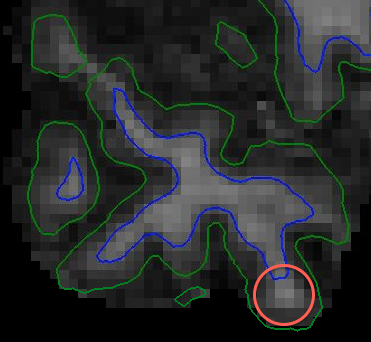
\includegraphics{wm_segmentation_error.png}}
\caption{Example of bad white matter segmentation. A cluster of white matter voxels
are classified as grey matter. It is difficult to see here, but the circled
white matter voxels have intensity values well below the expected value,
110.}\end{figure}


\subsection{Skull segmented as grey matter}
\label{surface_reconstruction:skull-segmented-as-grey-matter}
The skull stripping step can sometimes fail to remove parts of the skull or
dura, especially around the eyes, around orbitofrontal cortex, and near the top
of the head. This extra skull can sometimes get mislabeled as grey matter,
which you'll have to fix by erasing the voxels manually. For a full description
of the steps to take, see the \href{https://surfer.nmr.mgh.harvard.edu/fswiki/FsTutorial/SkullStripFix\_freeview}{Freesurfer skull-strip fix tutorial}\footnote{https://surfer.nmr.mgh.harvard.edu/fswiki/FsTutorial/SkullStripFix\_freeview}.

\begin{notice}{note}{Note:}
Most of the time skull strip errors won't cause surface errors. No
need to do anything in this case. The surfaces are all we care about.
\end{notice}
\begin{figure}[htbp]
\centering
\capstart

\scalebox{0.400000}{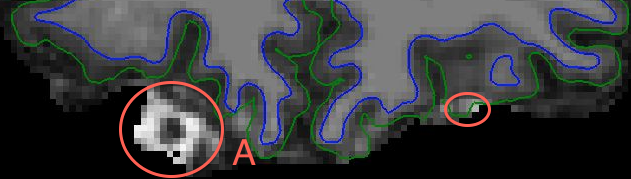
\includegraphics{skullstrip_nofix.png}}
\caption{Skull strip errors that don't affect the cortical surface.}\end{figure}


\subsection{White Matter Lesions}
\label{surface_reconstruction:white-matter-lesions}
We sometimes see subjects with small lesions scattered in their white matter.
These lesions look like dark spots in the white matter volume. They are more
common in older subjects, and usually having one means having many. When these
lesions occur near the grey/white matter boundary, they can cause the white
surface to errantly ``dip'' into (what should be) white matter.

Adding control points won't help in this situation. You can only use control
points to correct intensity issues due to scanner bias. Putting a control point
on a voxel tells Freesurfer ``This voxel is white matter, so you should scale
it's intensity (and that of neighboring voxels) to match other white matter
voxels.'' Since lesion voxels don't actually contain white matter, adding
control points here is the wrong choice. Instead, you will have to manually
fill in the lesion area in the subject's wm.mgz volume. For complete
instructions, see the \href{https://surfer.nmr.mgh.harvard.edu/fswiki/FsTutorial/WhiteMatterEdits\_freeview}{Freesurfer white-matter edit tutorial}\footnote{https://surfer.nmr.mgh.harvard.edu/fswiki/FsTutorial/WhiteMatterEdits\_freeview}.
\begin{figure}[htbp]
\centering
\capstart

\scalebox{0.400000}{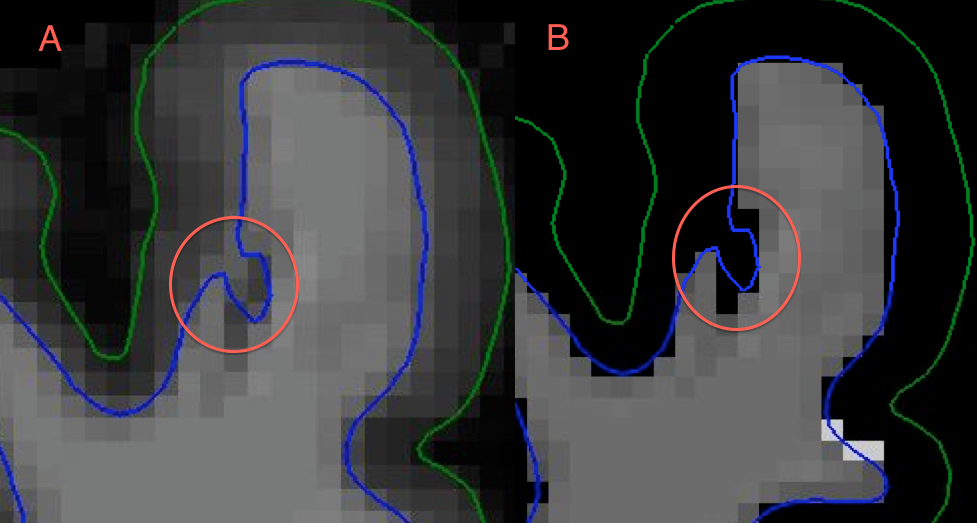
\includegraphics{wmlesion1.png}}
\caption{A white matter lesion causing a reconstruction error. \textbf{(A)} The error shown
on the brainmask.mgz volume. \textbf{(B)} The error shown on the wm.mgz volume. Note
how implausible the surface curvature is here. Also, see that the error is
more obvious in \textbf{(B)} than in \textbf{(A)}.}\end{figure}


\subsection{Midline weirdness}
\label{surface_reconstruction:midline-weirdness}
The paths that the surfaces take through the midline structures and the corpus
callosum are usually pretty nonsensical. \textbf{This is to be expected.} Don't
worry about it. The lines here are more or less arbitrary, since there is no
cortex to follow.
\begin{figure}[htbp]
\centering
\capstart

\scalebox{0.400000}{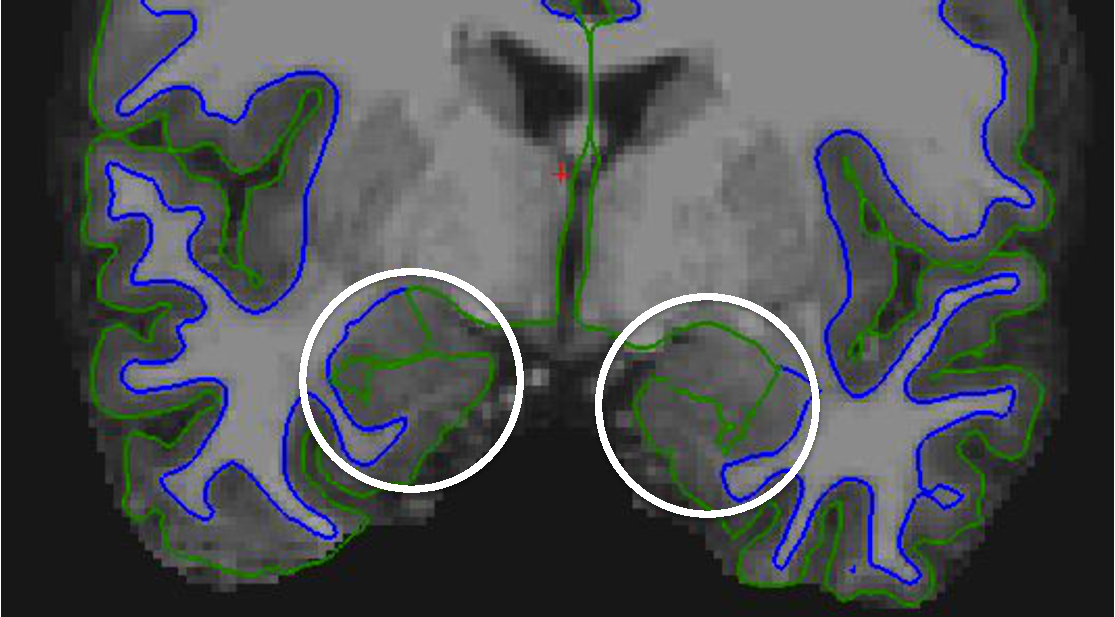
\includegraphics{midline_surf_inacc_02.pdf}}
\caption{Uninterpretable pial surface through midline subcortical structures.}\end{figure}


\section{Quality control record keeping}
\label{surface_reconstruction:freesurfer-white-matter-edit-tutorial}\label{surface_reconstruction:quality-control-record-keeping}
It's very important to take notes while inspecting your data. This way you can
return months later and feel confident that the quality assurance was done
right. As a lab, we try to stick to a common format for quality control record
keeping.

The quality control spreadsheet, usually called \emph{recon\_QC.xls} has two tabs.
The first tab, called \emph{Recon check}, is for keeping track of who checked which
subjects when, and whether the reconstruction was ok, or required fixing.

\begin{tabulary}{\linewidth}{|L|L|L|L|}
\hline
\textsf{\relax 
Subject
} & \textsf{\relax 
Recon OK
} & \textsf{\relax 
Date
} & \textsf{\relax 
Checked by
}\\
\hline
BSYN\_CB\_02
 & 
yes
 & 
8/4/15
 & 
CL
\\

BSYN\_S\_02
 & 
no
 & 
8/4/15
 & 
CL
\\
\hline\end{tabulary}


The second tab, called \emph{Recon errors}, is for keeping track of errors that you
find in the surface reconstruction. Each row corresponds to an error. In the
columns, you record the subject that you found the error in, a description of
the error, the voxel coordinates for the error, what fix you applied (if any)
and whether the fix worked. Keep in mind that this sheet is both for errors
that need intervention, and for problem spots you just want to note, but don't
need any further action. If you're not sure how to describe an error you see,
or how to fix it, you should still take down at least the voxel coordinates.
This way you can return to it later.

\begin{tabulary}{\linewidth}{|L|L|L|L|L|}
\hline
\textsf{\relax 
Subject
} & \textsf{\relax 
Error
} & \textsf{\relax 
Coordinates
} & \textsf{\relax 
Fix
} & \textsf{\relax 
Fixed
}\\
\hline
BSYN\_CB\_02
 & 
Questionable partial-volume decision
 & 
{[}87, 153, 87{]}
 & 
N/A
 & 
N/A
\\

BSYN\_S\_02
 & 
Skull included around right eye
 & 
{[}154, 144, 175{]}
 & 
N/A
 & 
N/A
\\

BSYN\_S\_02
 & 
Skull included in right orbital frontal
 & 
{[}160, 151, 156{]}
 & 
Removed extra skull
 & 
yes
\\
\hline\end{tabulary}



\section{Post reconstruction processing}
\label{surface_reconstruction:post-reconstruction-processing}
After Freesurfer reconstruction is complete, some additional surface processing
is required before you can move on to later analysis steps. These steps are
carried out using the \code{postrecon} script, and include:
\begin{itemize}
\item {} 
Nonlinear registration of the subject's T1.mgz with the MNI 152 template
using FSL's \code{fsl\_anat}.

\item {} 
Converting primary surfaces to Gifti format using \code{mris\_convert}.

\item {} 
Constructing HCP-style midthickness and inflated surfaces using \code{wb\_command
-surface-average} and \code{wb\_command -surface-generate-inflated}.

\item {} 
Downsampleing Gifti surfaces to the 32k\_fs\_LR mesh using \code{wb\_command
-surface-resample}. This reduces number of vertices from \textgreater{}100K to \textasciitilde{}32K.
After downsampling, each surface face occupies \textasciitilde{}2mm$^{\text{2}}$, which more
closely follows the resolution of the raw data.

\end{itemize}

\code{postrecon} only requires a subject ID argument:

\begin{Verbatim}[commandchars=\\\{\}]
postrecon \PYG{n+nv}{\PYGZdl{}subj}
\end{Verbatim}

Subject folders are modified in place. The results of the volumetric
registration are written to mri/T1. The generated surfaces are added to the
surf folder.



\renewcommand{\indexname}{Index}
\printindex
\end{document}
